%*----------- SLIDE -------------------------------------------------------------

\begin{frame}[c]{} 
    \framesubtitle{}
    \transdissolve[duration=0.5]
   
    \begin{center}
        \Wider{%
        \begin{shaded}
        \begin{center}
            \vspace*{0.5cm}
            \resizebox{!}{0.5cm}{%
                \color{bg} Projetos
            }%
        \end{center}
        \end{shaded}
        }%
    \end{center}

\end{frame}






\begin{frame}[t]{turBOT}

    Objetivo é desenvolver um AUV pequeno para operar em águas razas
    \begin{center}

    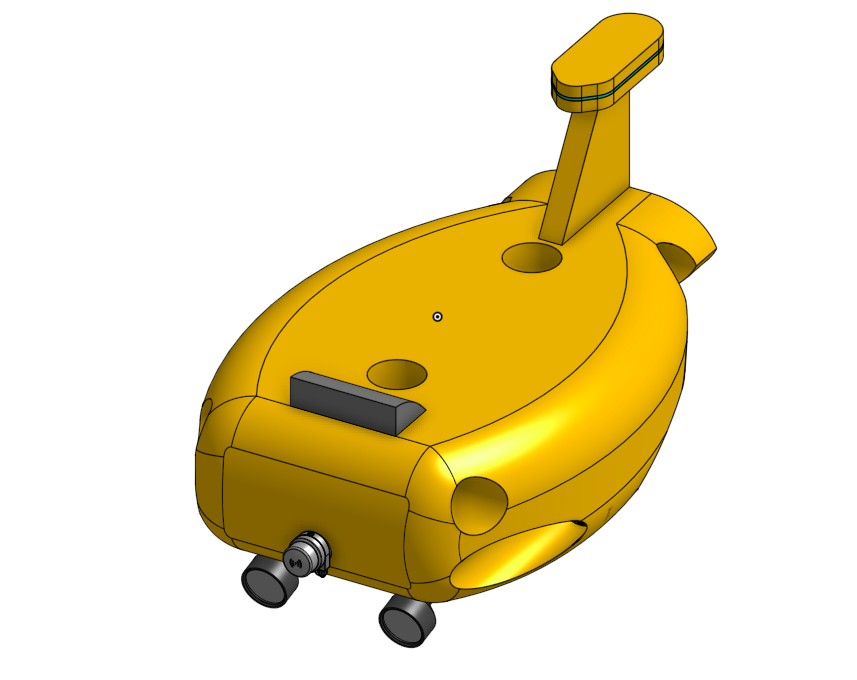
\includegraphics[width=0.5\textwidth]{turbot.png}

    \end{center}
    
    
            
\end{frame}

\begin{frame}[t]{turBOT}

    Desenvolvimento de um veículo submarino para atuar em águas rasas para fins exploratórios,
    o veículo em desenvolvimento terá capacidade de identificar algumas anomalias ou padrões construídos
    e disponibilizará para os pesquisadores, apresenta uma dimensão menor do que os veículos comerciais.
    \begin{figure}
    \begin{center}

    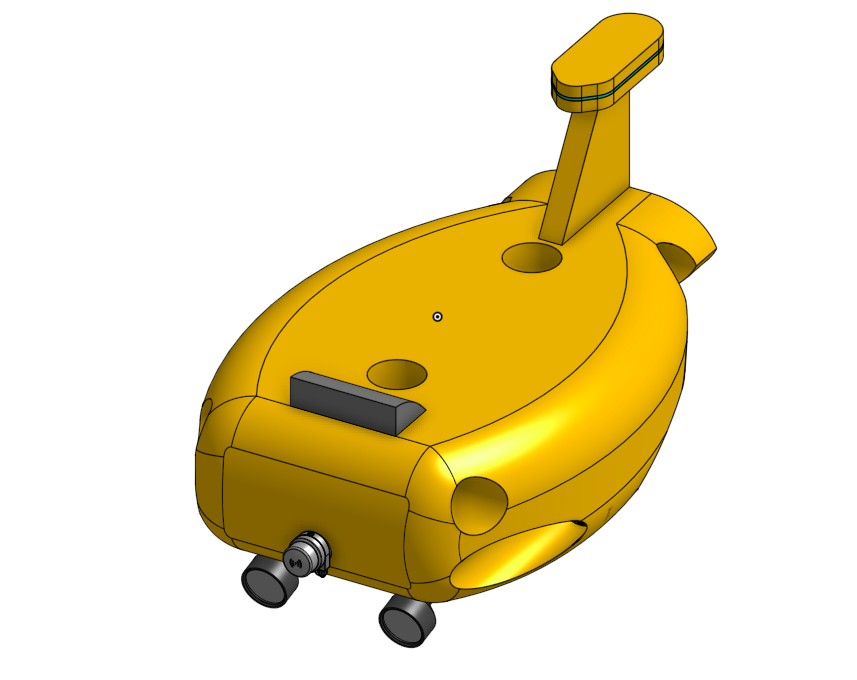
\includegraphics[width=0.5\textwidth]{turbot.png}

    \end{center}
    
    
            
\end{frame}

\begin{frame}[t]{turBOT - Metodologia}

    
    \begin{center}

    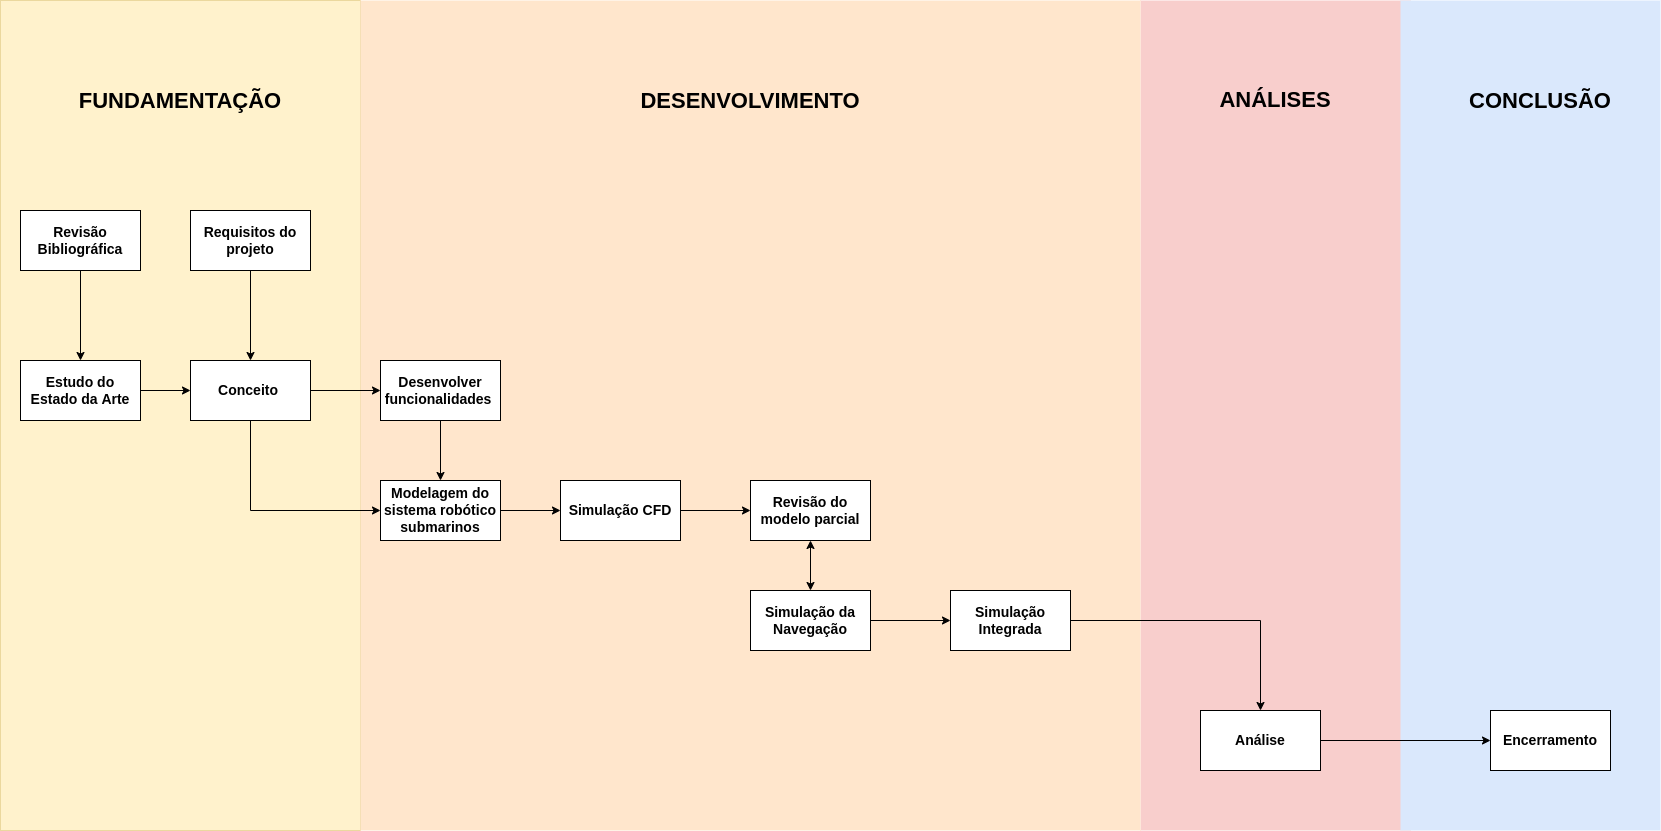
\includegraphics[width=0.5\textwidth]{metodolodia2.png}

    \end{center}
    
    
            
\end{frame}

%*----------- SLIDE -------------------------------------------------------------
\begin{frame}[t]{Desenvolvido no projeto}
    \begin{itemize}
        \item Elaborado o cronograma do projeto
        \item Realizado o método BiLi
        \item Estudos sobre linguagens de programação C++, Python e R
        \item Estudo ROS e openFOAM
        \item Estudo sobre CFD (Fluidodinâmica computacional)
    \end{itemize}    
%*----------- notes
    \note[item]{Notes can help you to remember important information. Turn on the notes option.}
\end{frame}
%-
%*----------- SLIDE -------------------------------------------------------------
\begin{frame}[t]{Próximos passos do projeto}
    \begin{itemize}
        \item Listar as funcionalidades para desenvolvimento da montagem do sistema robótico submarino
        \item Simulação no OpenFOAM
        \item Simulação no ROS
        \item Desenvolvimento de 4 artigos: 
        \begin{itemize}
            \item[] 2022- SOTA e Simulação OpenFOAM
            \item[] 2023- DOE OpenFOAM e ROS 
        \end{itemize}   
        
    \end{itemize}    
%*----------- notes
    \note[item]{Notes can help you to remember important information. Turn on the notes option.}
\end{frame}



\begin{frame}[t]{FlatFish@ROS}

    
    Este projeto teme como alvo trazer as funcionalidades do FlatFISH para operar em ROS
    \begin{center}

    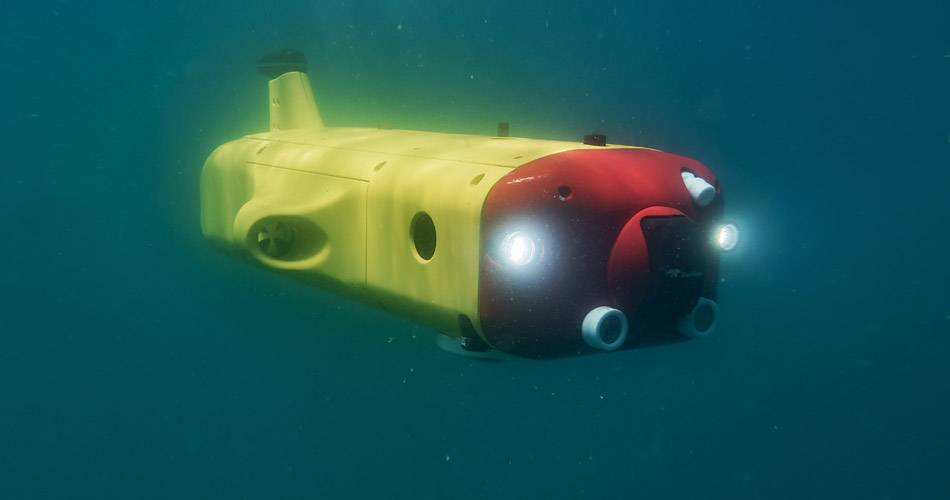
\includegraphics[width=0.5\textwidth]{flatfish.jpg}

    \end{center}
    
    
            
\end{frame}


\begin{frame}[t]{Pirabots}

    
    O foco é implmentar ações autônomas em ROVs: BlueROV e BirROV.

    \begin{columns}
        \column{.45\linewidth}
    \begin{center}

        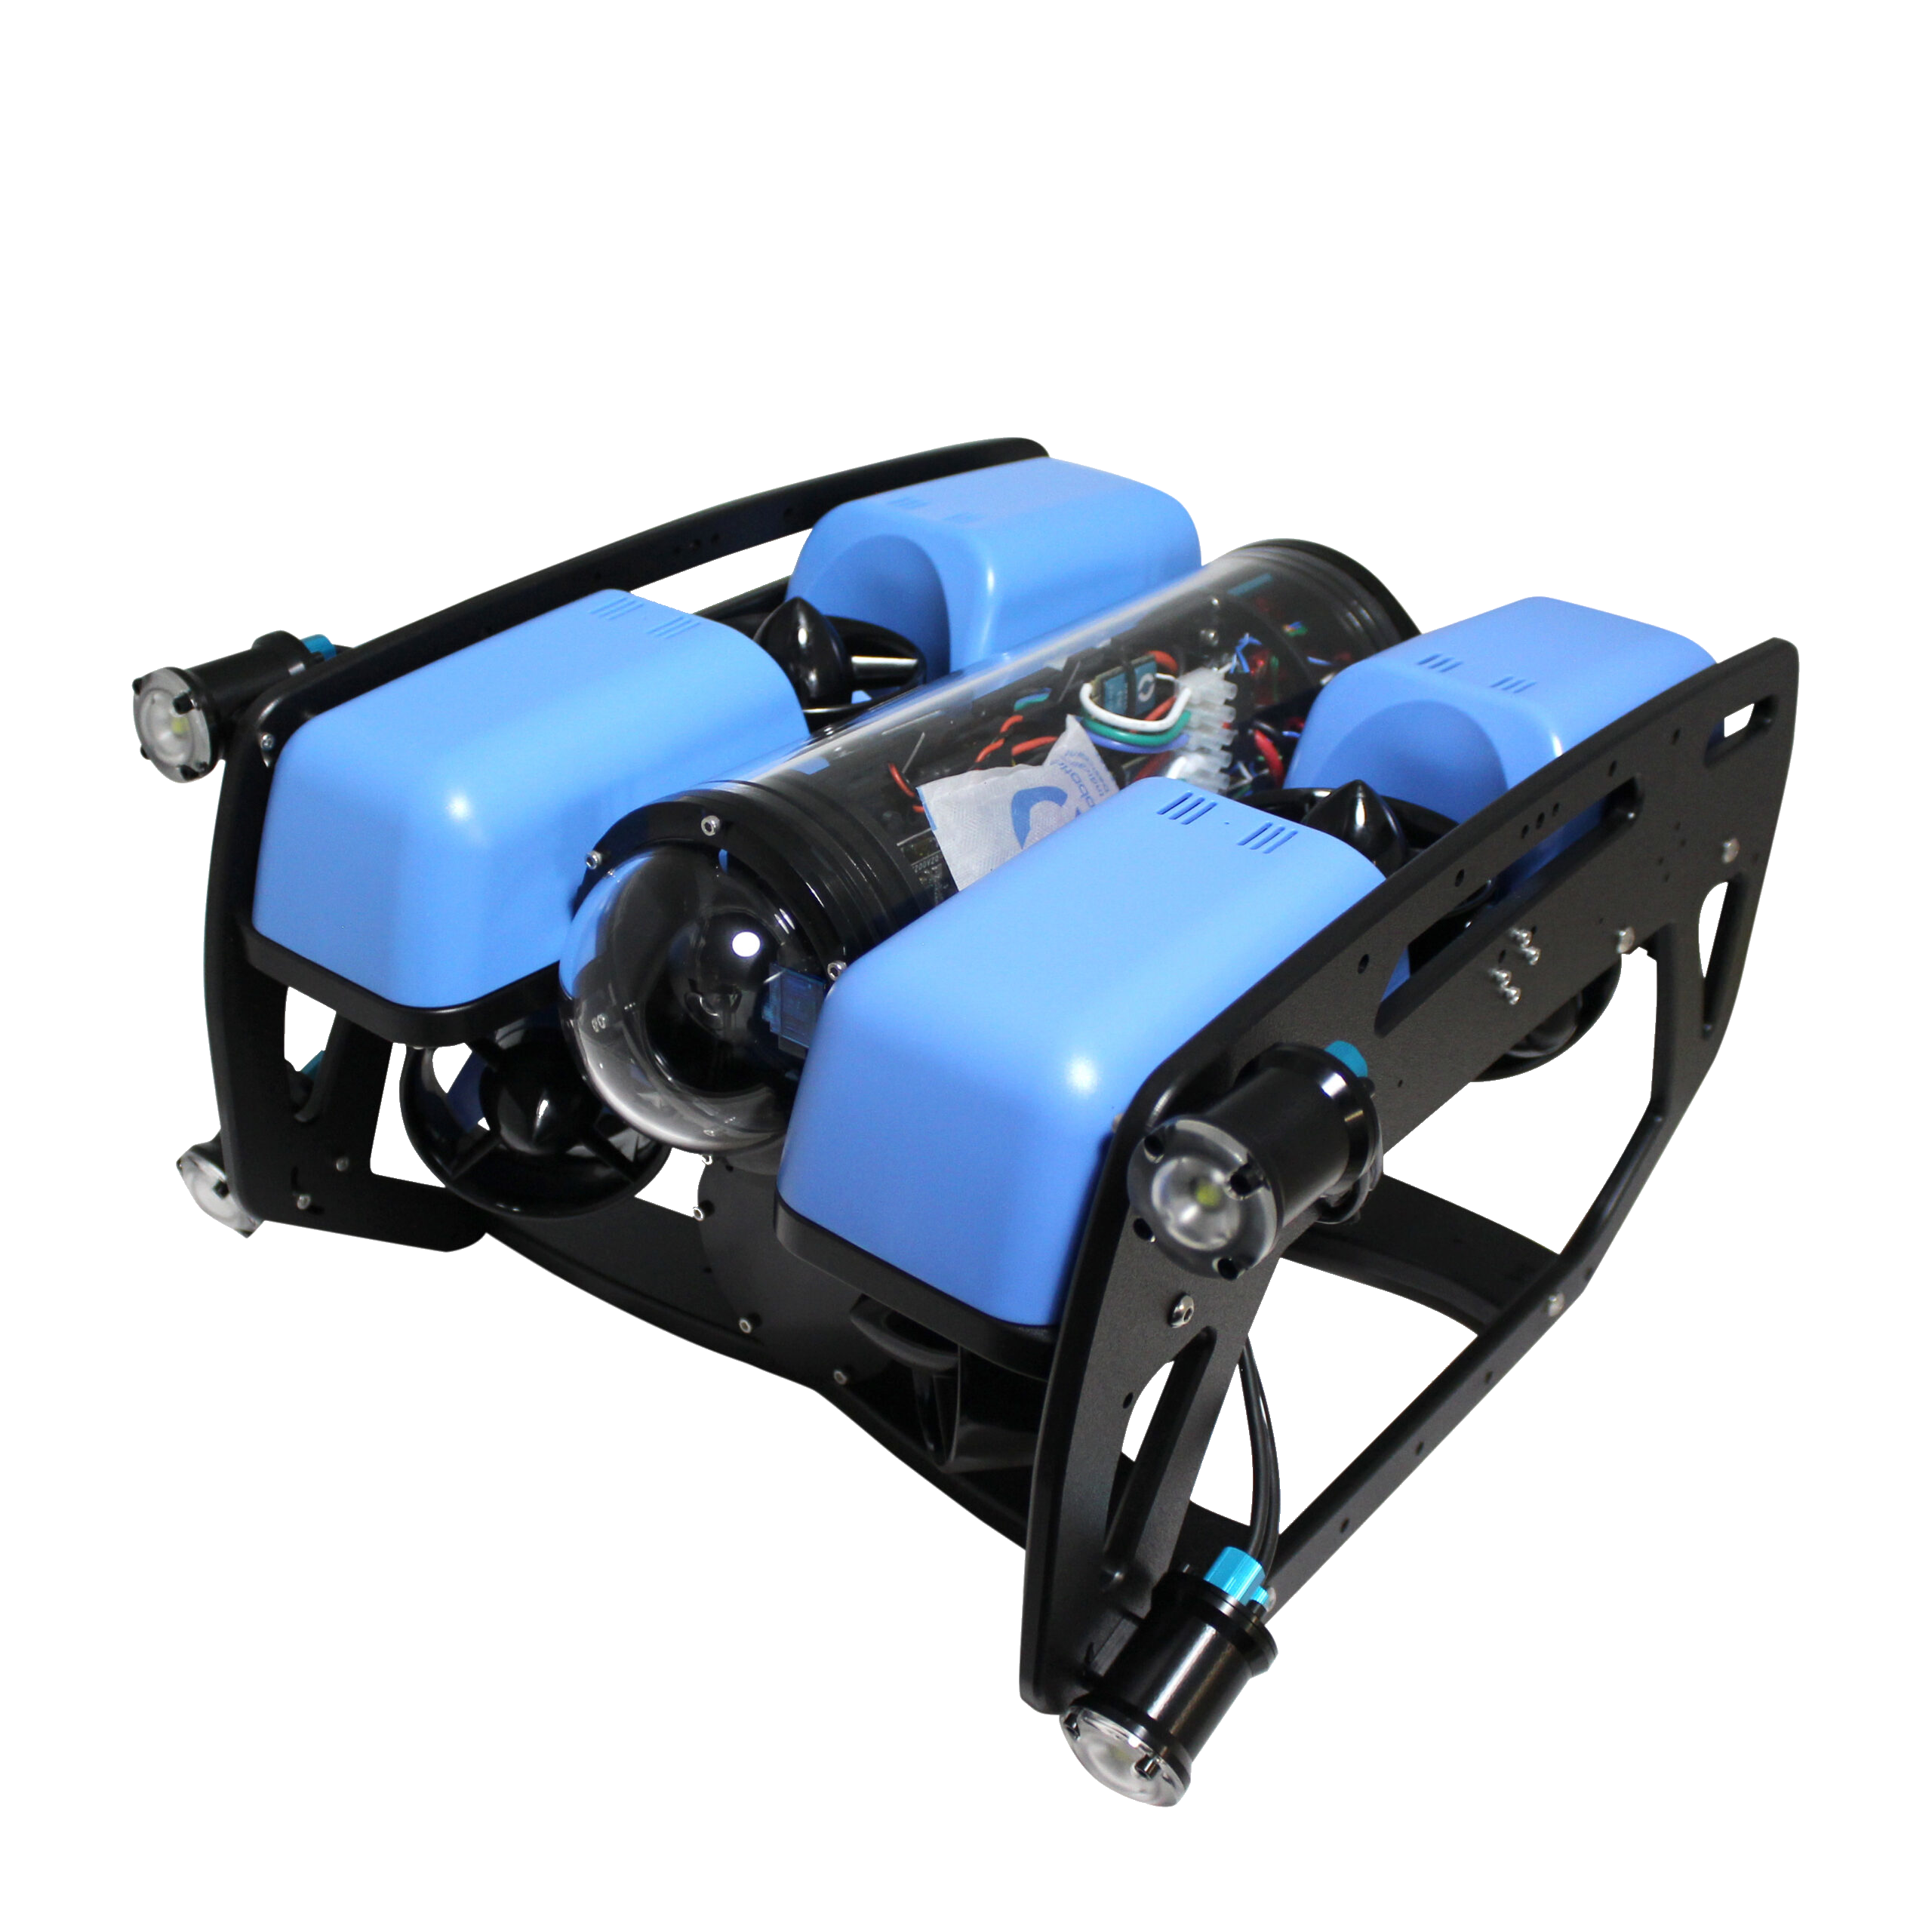
\includegraphics[width=0.8\textwidth]{bluerov.png}

    \end{center}

    \column{.45\linewidth}
    \vspace*{0.3cm}
    \begin{center}

        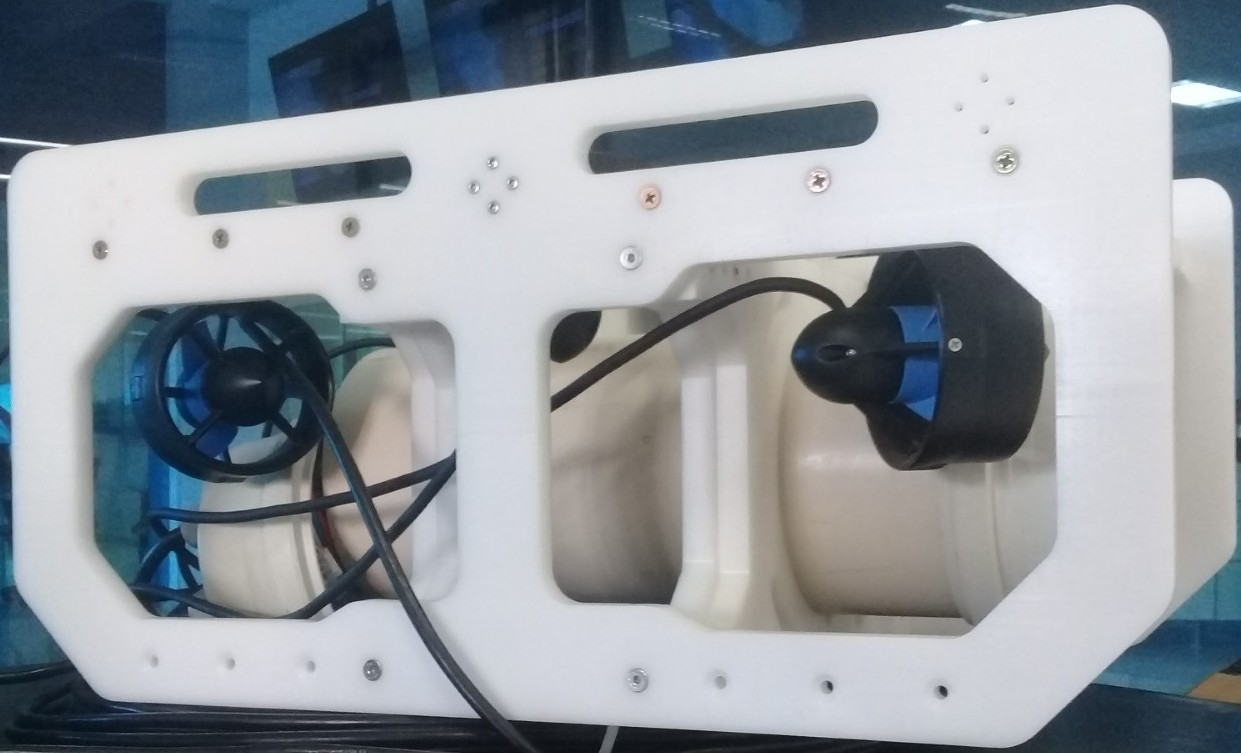
\includegraphics[width=0.8\textwidth]{bir_rov.jpg}

    \end{center}

\end{columns}

\end{frame}




\begin{frame}[t]{Challenges}

   
Pipeline identification - Solo

Pipeline Following - In Group
\vspace*{0.1cm}
\begin{center}

    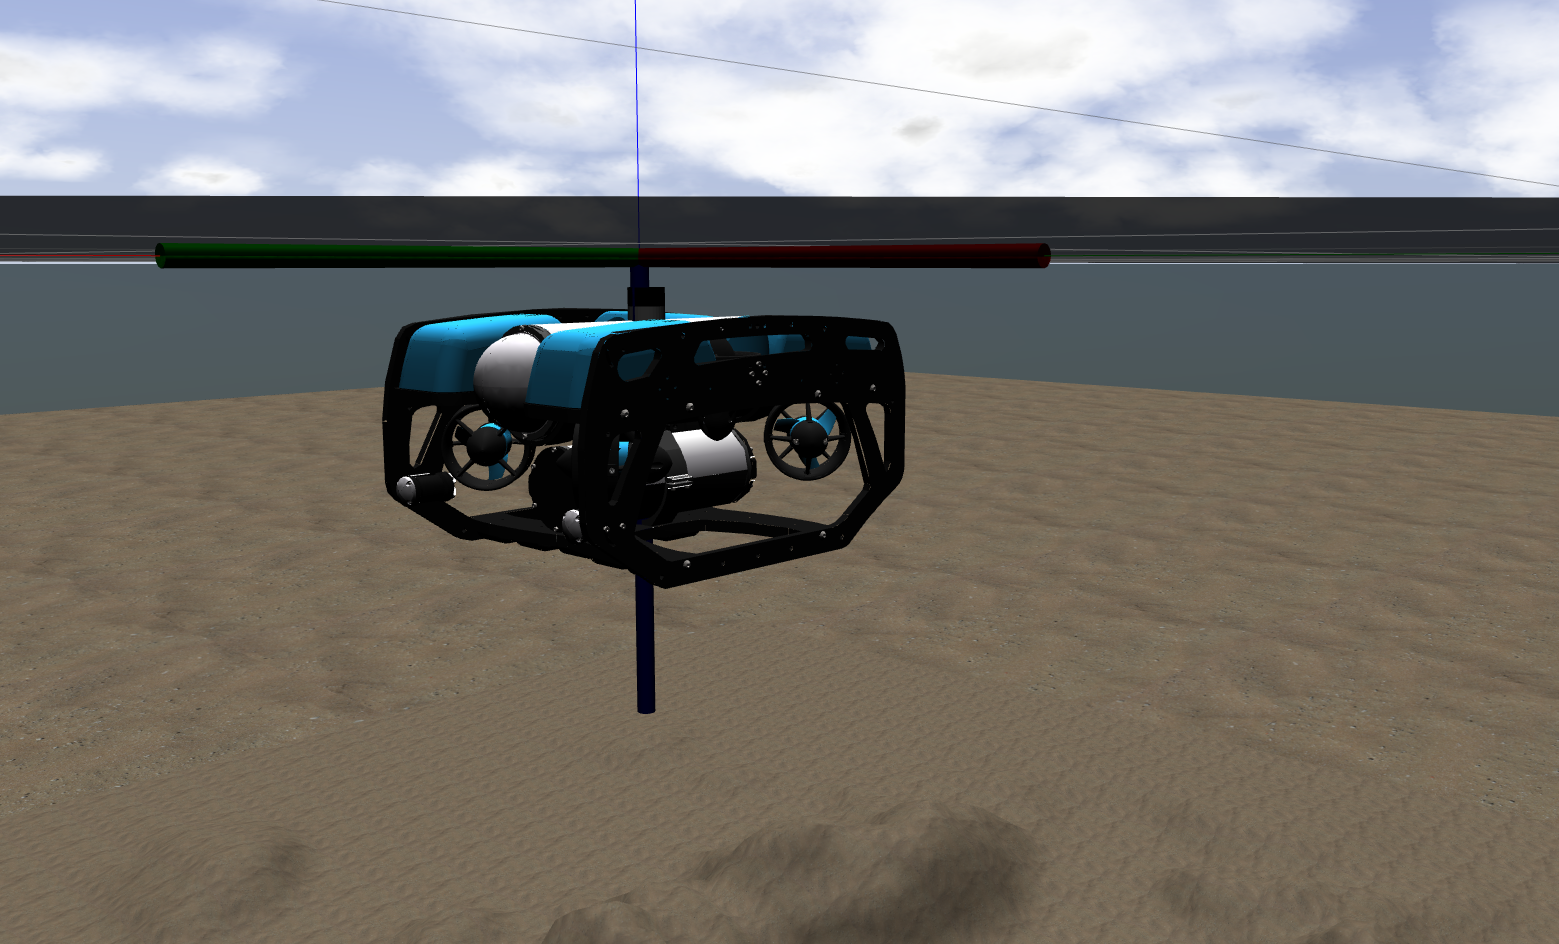
\includegraphics[width=0.55\textwidth]{bluerov2_uuv_simulator.png}

\end{center}
    
    
            
\end{frame}



    \begin{frame}[t]{Members}
        %\transboxin[duration=1,direction=30]
       
        \newline
       
        Os atuais membros da linha de pesquisa saõ:
    
        \\
        \\
        \\
    
        \\
    
        \vspace*{1cm}
    
        \begin{columns}[c]
                
            \column{0.33\linewidth}
    
            
          
    
            \begin{center}
                \begin{figure}
                    %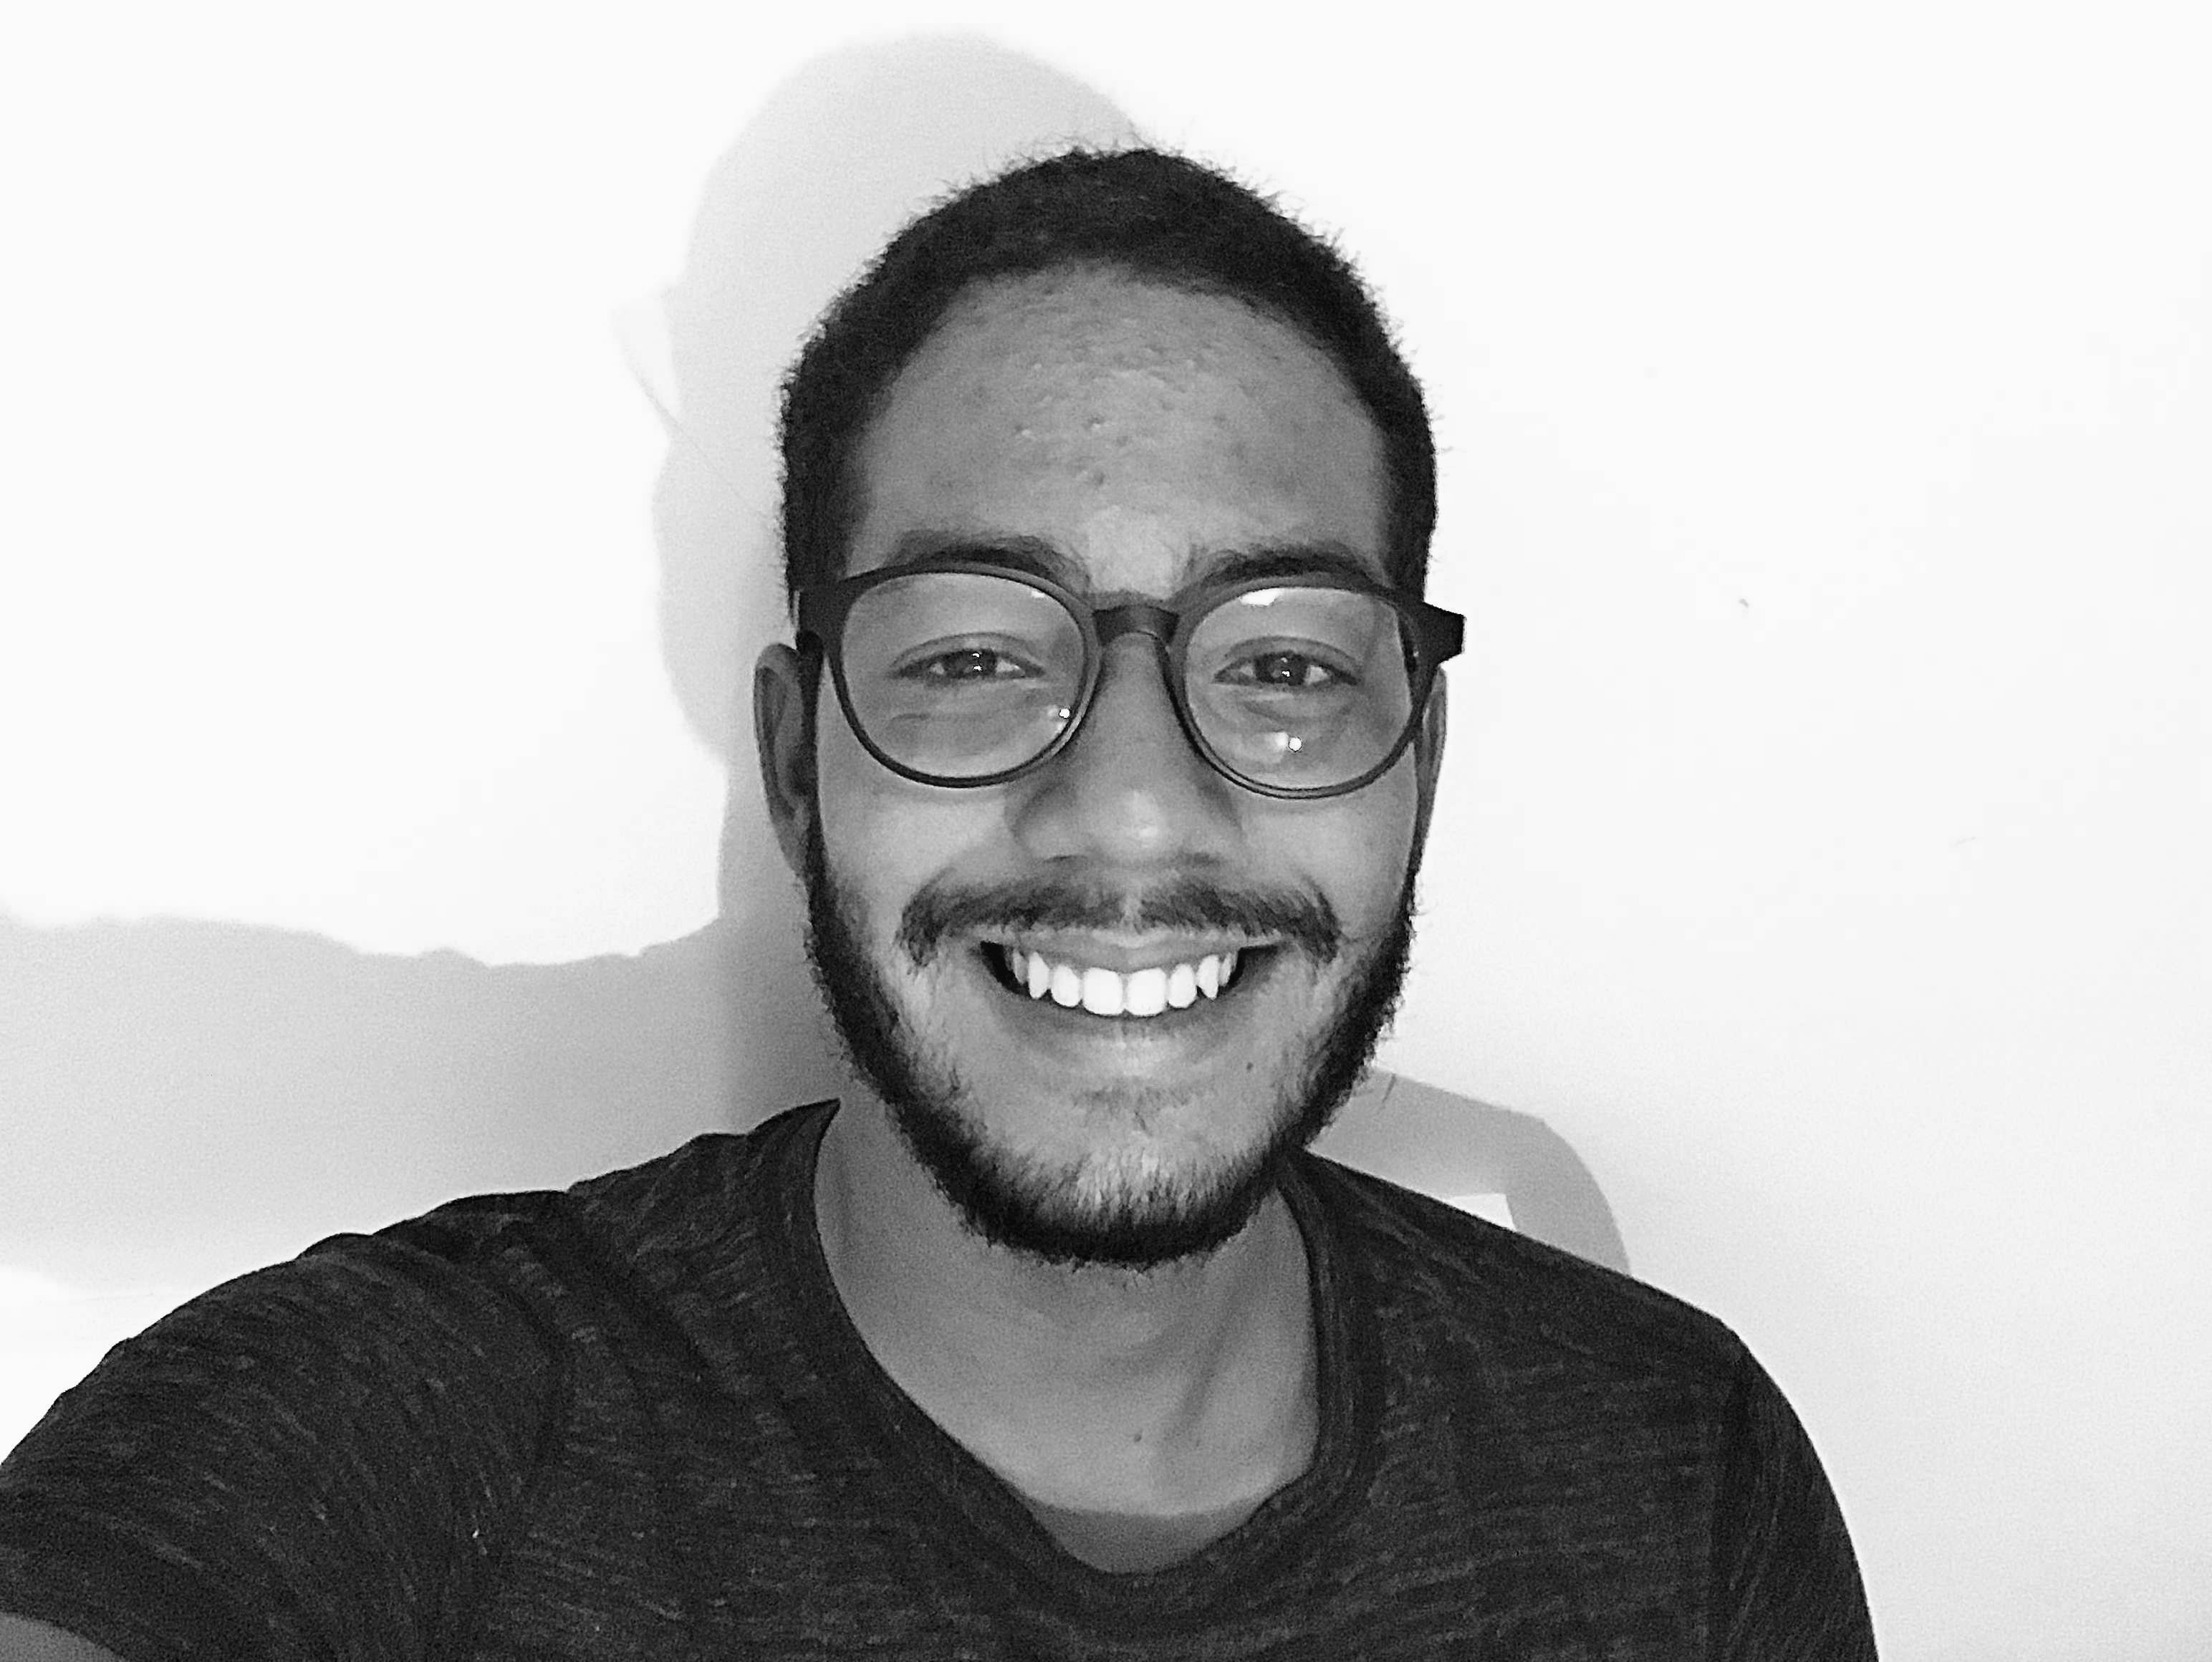
\includegraphics[width=0.45\textwidth]{alexandre.png}
                    \roundpic[xshift=0cm,yshift=0cm]{1.915cm}{2.5cm}{alexandre}
                    \caption{Alexandre Adonai}
                \end{figure}
            \end{end}
    
            \column{0.33\linewidth}
    
            \begin{center}
                \begin{figure}
                    
                    \roundpic[xshift=0cm,yshift=0cm]{2.0cm}{2.5cm}{matheus1}
                    \caption{Matheus Anselmo}
                \end{figure}
            \end{end}
    
    
            \column{0.33\linewidth}
            \begin{center}
                \begin{figure}
                    \roundpic[xshift=0cm,yshift=0cm]{2.0cm}{2.5cm}{tamara}
                \caption{Tâmara Lins}
            \end{figure}
        \end{end}
    
        \end{columns}
       
    \end{frame}


%-
%-
%*-